\chapter{Results and Interpretation}

%%%%%%%%%%%%%%%%%
%     2016
%%%%%%%%%%%%%%%%%
\section{2016 Datasets}

\subsection{Primary Analysis}
In order to roughly understand a group (similar patterns) of data, one way to do it is to reduce the dimension of data. In our case, there are 259 features which will be transformed into two dimension on the basis of two eigenvectors (selected by two largest eigenvalues) belonging to covariance matrix which computed from the datasets.
\begin{figure}[h!]
    \centering
    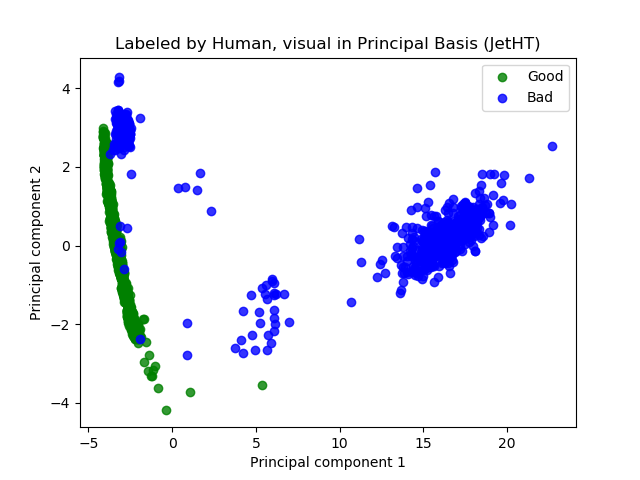
\includegraphics[width=0.6\textwidth]{images/reco/2016/JetHT_label_2016.png}
    \caption{Principal component with the labeled color from the system}
    \label{fig:JetHT_label_2016}
\end{figure}

As you could see on the green line in Figure \ref{fig:JetHT_label_2016} that there are nice band which is good LS and a few weird LSs that located outside the tubular shape as well as bad LS that could be divided into the bad LS with some patterns and anamaly bad LS which I would called both of them as "outlier". That's essentially the punchline why I called outlier detection instead of anomaly detection.

\subsection{Performance}
We Iteratively retrain the model ten times to make sure that it's working systematically and plot the root mean square as a shady fluctuation in Figure \ref{fig:performance_2016}
\begin{figure}[h!]
\centering
    \begin{subfigure}[b]{0.49\linewidth}
        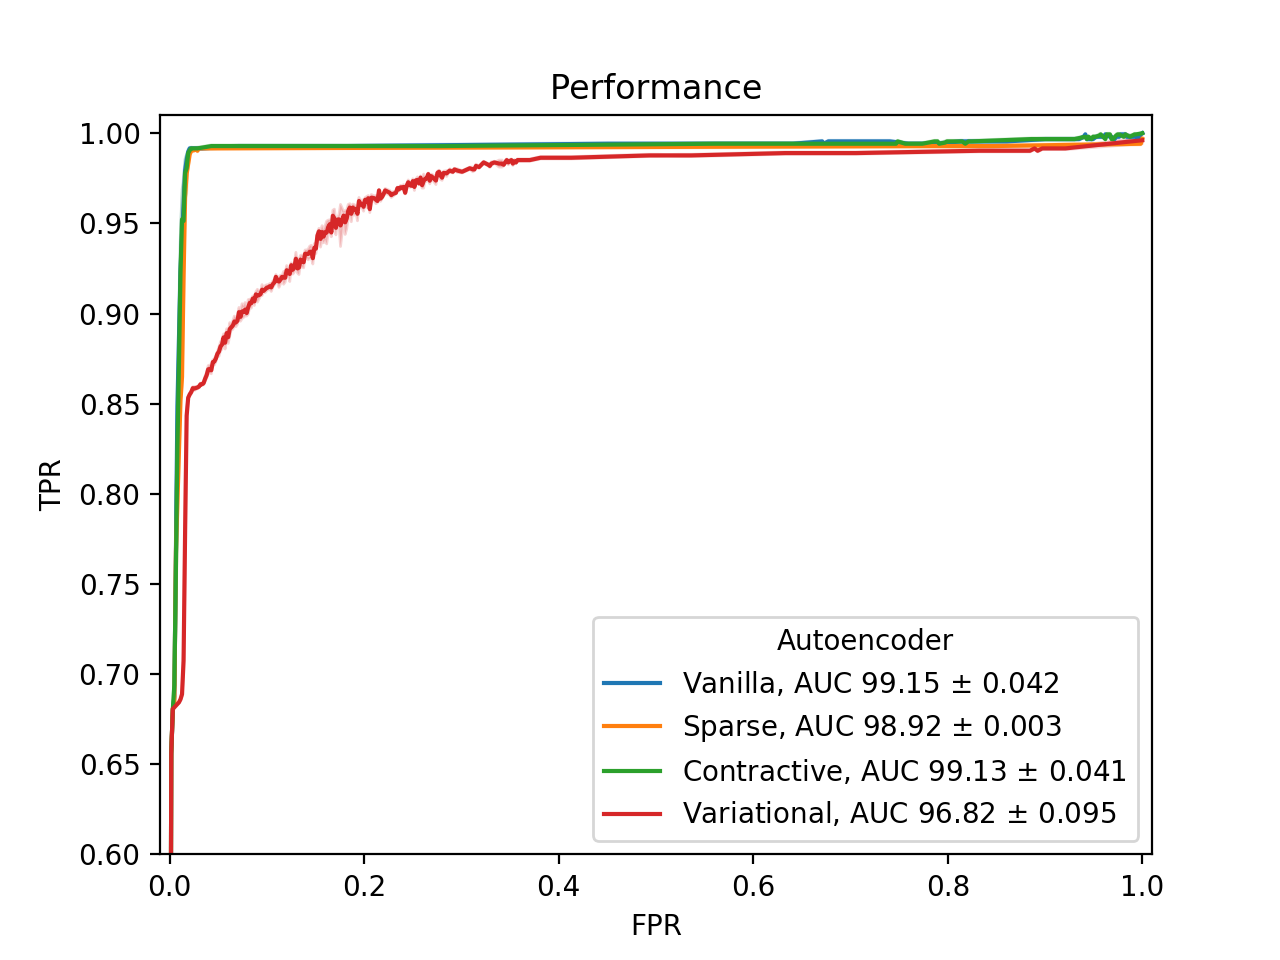
\includegraphics[width=\linewidth]{images/reco/2016/performance.png}
        \caption{4 Flavours of AE}
    \end{subfigure}
    \begin{subfigure}[b]{0.49\linewidth}
        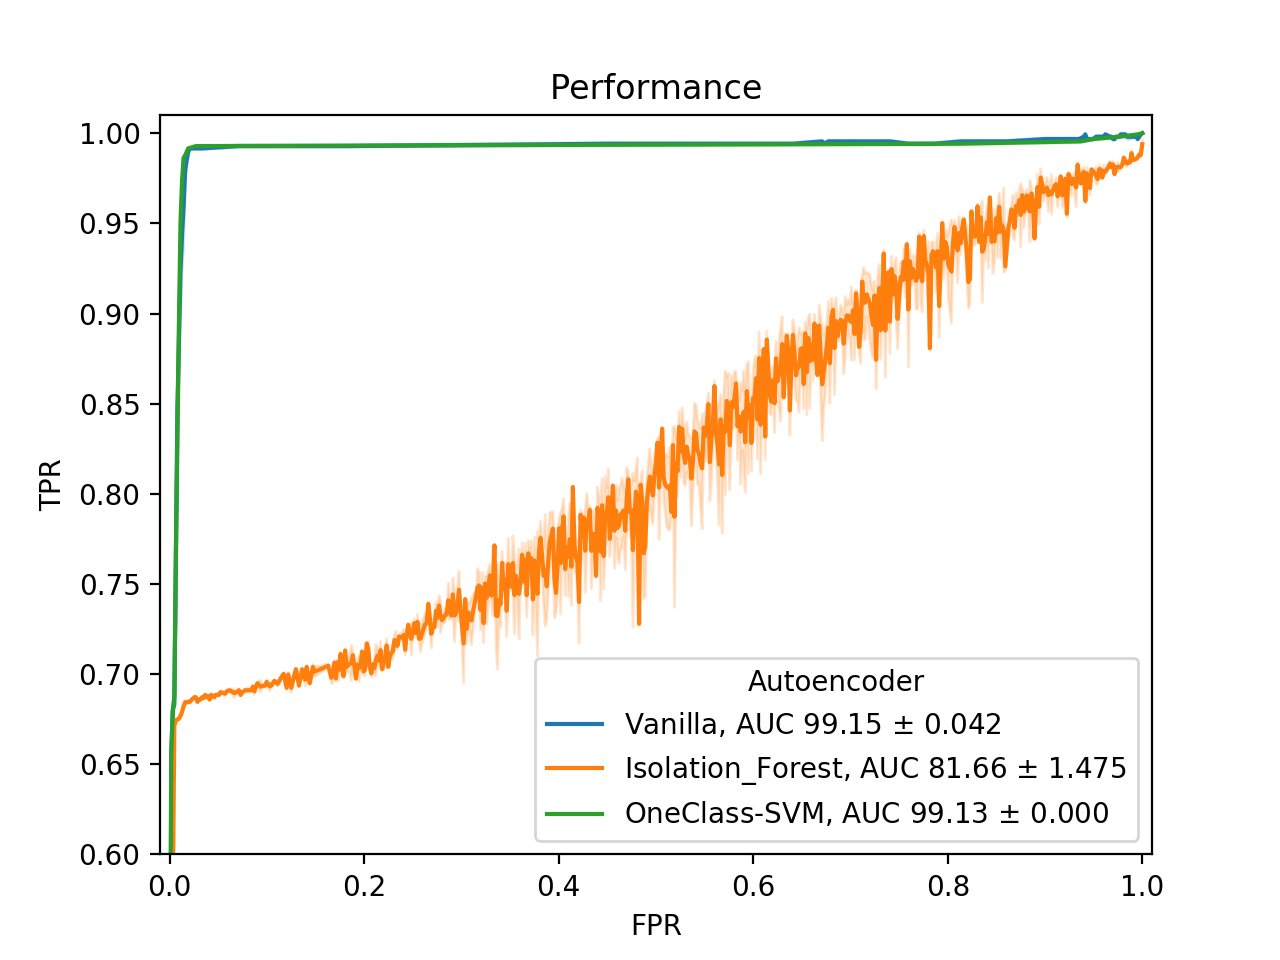
\includegraphics[width=\linewidth]{images/reco/2016/performance_ml.png}
        \caption{Vanilla AE vs SVM vs Isolation Forest}
    \end{subfigure}
\caption{Comparative visualization of model performance}
\label{fig:performance_2016}
\end{figure}

To sum up, even there are fancy mathematical expression of non-vanilla autoencoders but it does not guarantee that we would get the best performance out if it. On the other hand, simplest AE has the performance among all AE. One other intersting spot is the performance of OneClass-SVM also yield the remarkable results as nearly compatible with Vanilla AE without any fluctuation since the model itself has no randomness and working very strightforward.

\subsection{Distribution of decision value (to find the threshold)}
The story behind the performance figure is genuinely extracted from the distribution of decision value from Figure \ref{fig:2016_decision_value_dist} and slowly moving a threshold of minimal point in the overlapping region of good and bad LS from label in the distribution until it got the maximal value. The below figures are the comparison between our two great candidates by consider to pick some threshold and see the contamination in each side.

\begin{figure}[h!]
    \centering
    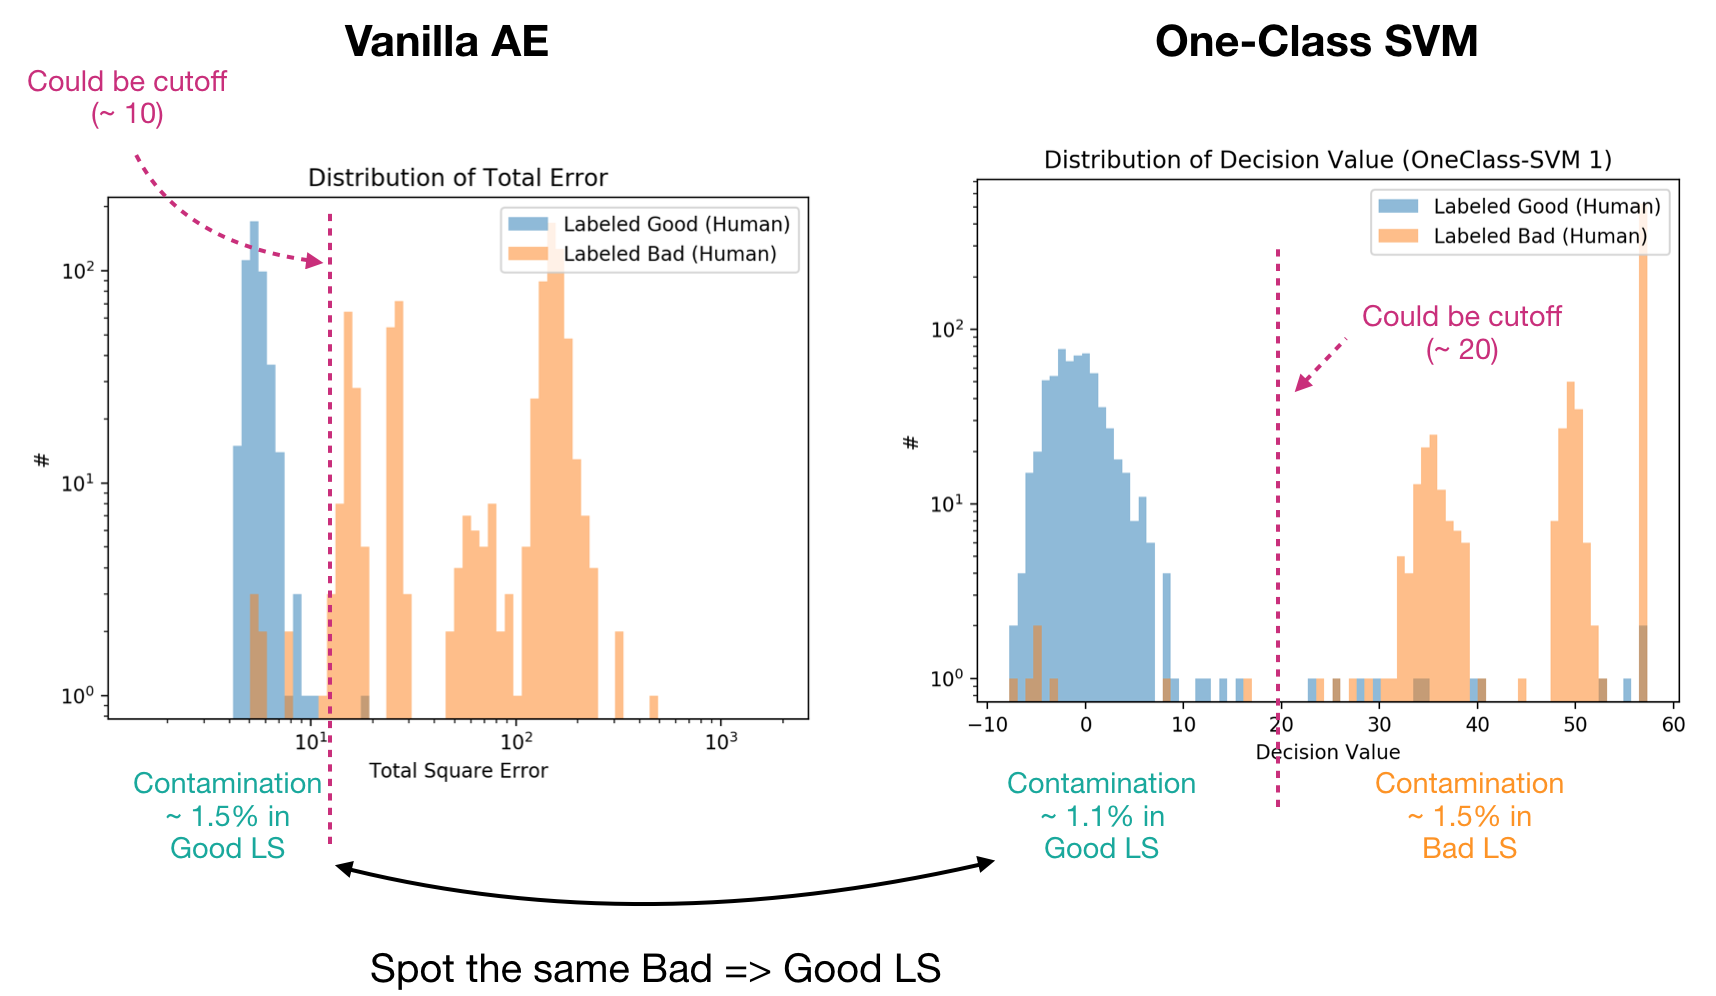
\includegraphics[width=\textwidth]{images/reco/2016/decision_value_dist.png}
    \caption{Distribution of decision value}
    \label{fig:2016_decision_value_dist}
\end{figure}

For Vanilla AE, the contamination of bad LS falling into good LS is around 1\% over the good LS below the cutoff and there are only countable of good LS falling into bad LS which might be ignorable.

For OneClass-SVM, the contamination LS that bad falling into good LS is almost exactly the same as Vanilla AE does. There is no coincidence for totally different approach of model train and spot the same thing. This might implicitly implies that it either came from some imperfection of data in the training and testing or some kind of malfunction in the sub-system couldn't propagated into JetHT physics objects.

As can be seen in the distribution, there is no clear grey zone for this study so far.

\subsection{Example of square error from reconstruction}
Figure \ref{fig:2016_example_se} show the example of LS reconstruction which calculated from x and x' between good and bad LS.
\begin{figure}[h!]
    \centering
    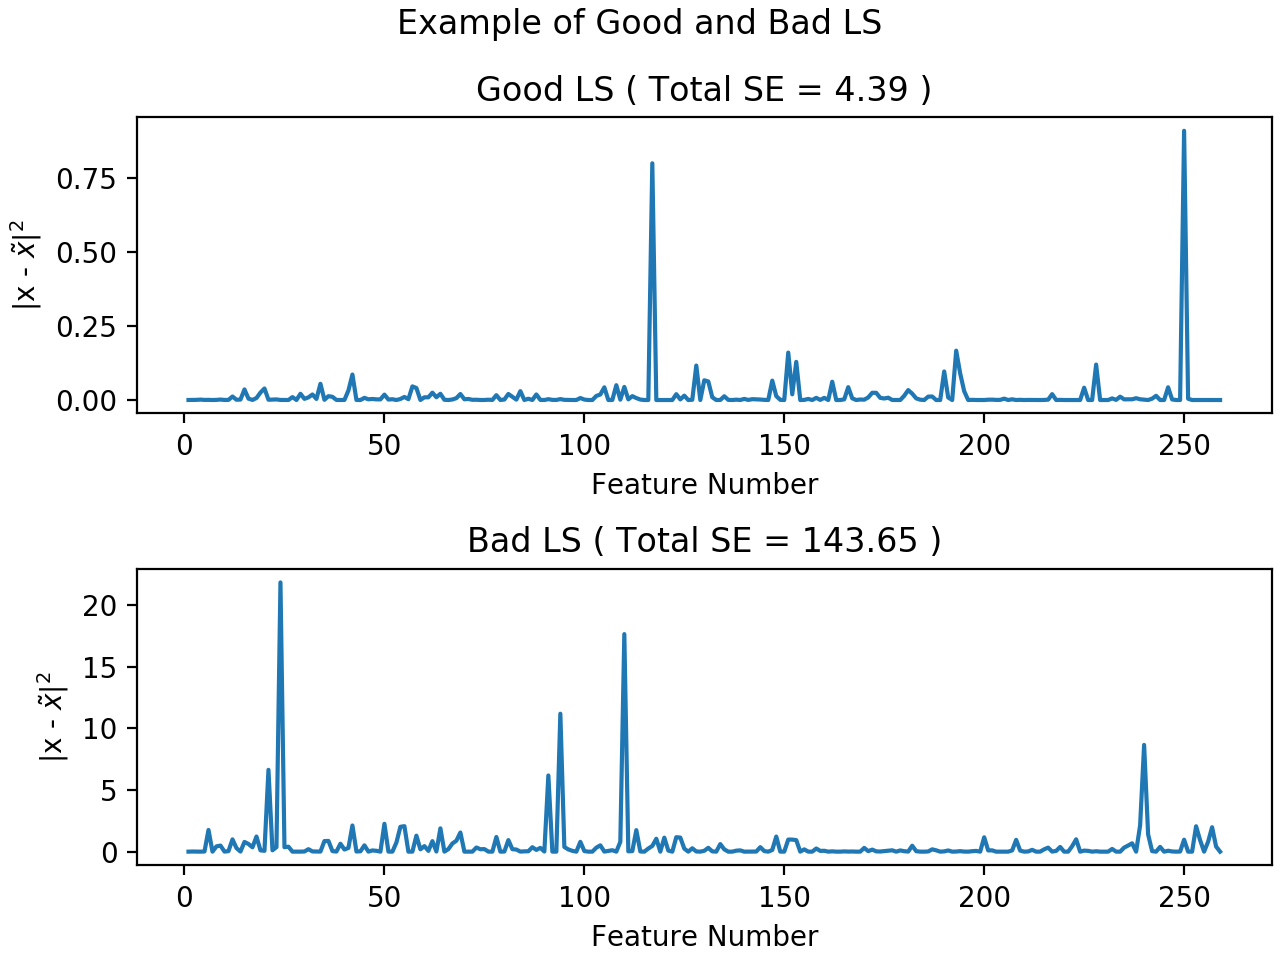
\includegraphics[width=0.8\textwidth]{images/reco/2016/example_se.png}
    \caption{Reconstruction error from Vanilla AE}
    \label{fig:2016_example_se}
\end{figure}

\subsection{Extended Investigation}
You might wondering why many of bad LS seems to have a group of bad LS as you have seen in the plot of hyperspace and few collection of bad LS in decision value distribution (As the black arrow that link between the distribution and 2D-hyperspace). In this section, I want to explicitly prove that the model really see that the right cluster is the worse bad LS and more closer to tubular is less bad LS which decision value have to be quite similar to good LS. In order to prove that, I choose our best candidate to shading the decision value as z-axis color to represent how bad LS in each data point is as in Figure \ref{fig:2016_guess_visual}.
\begin{figure}[h!]
    \centering
    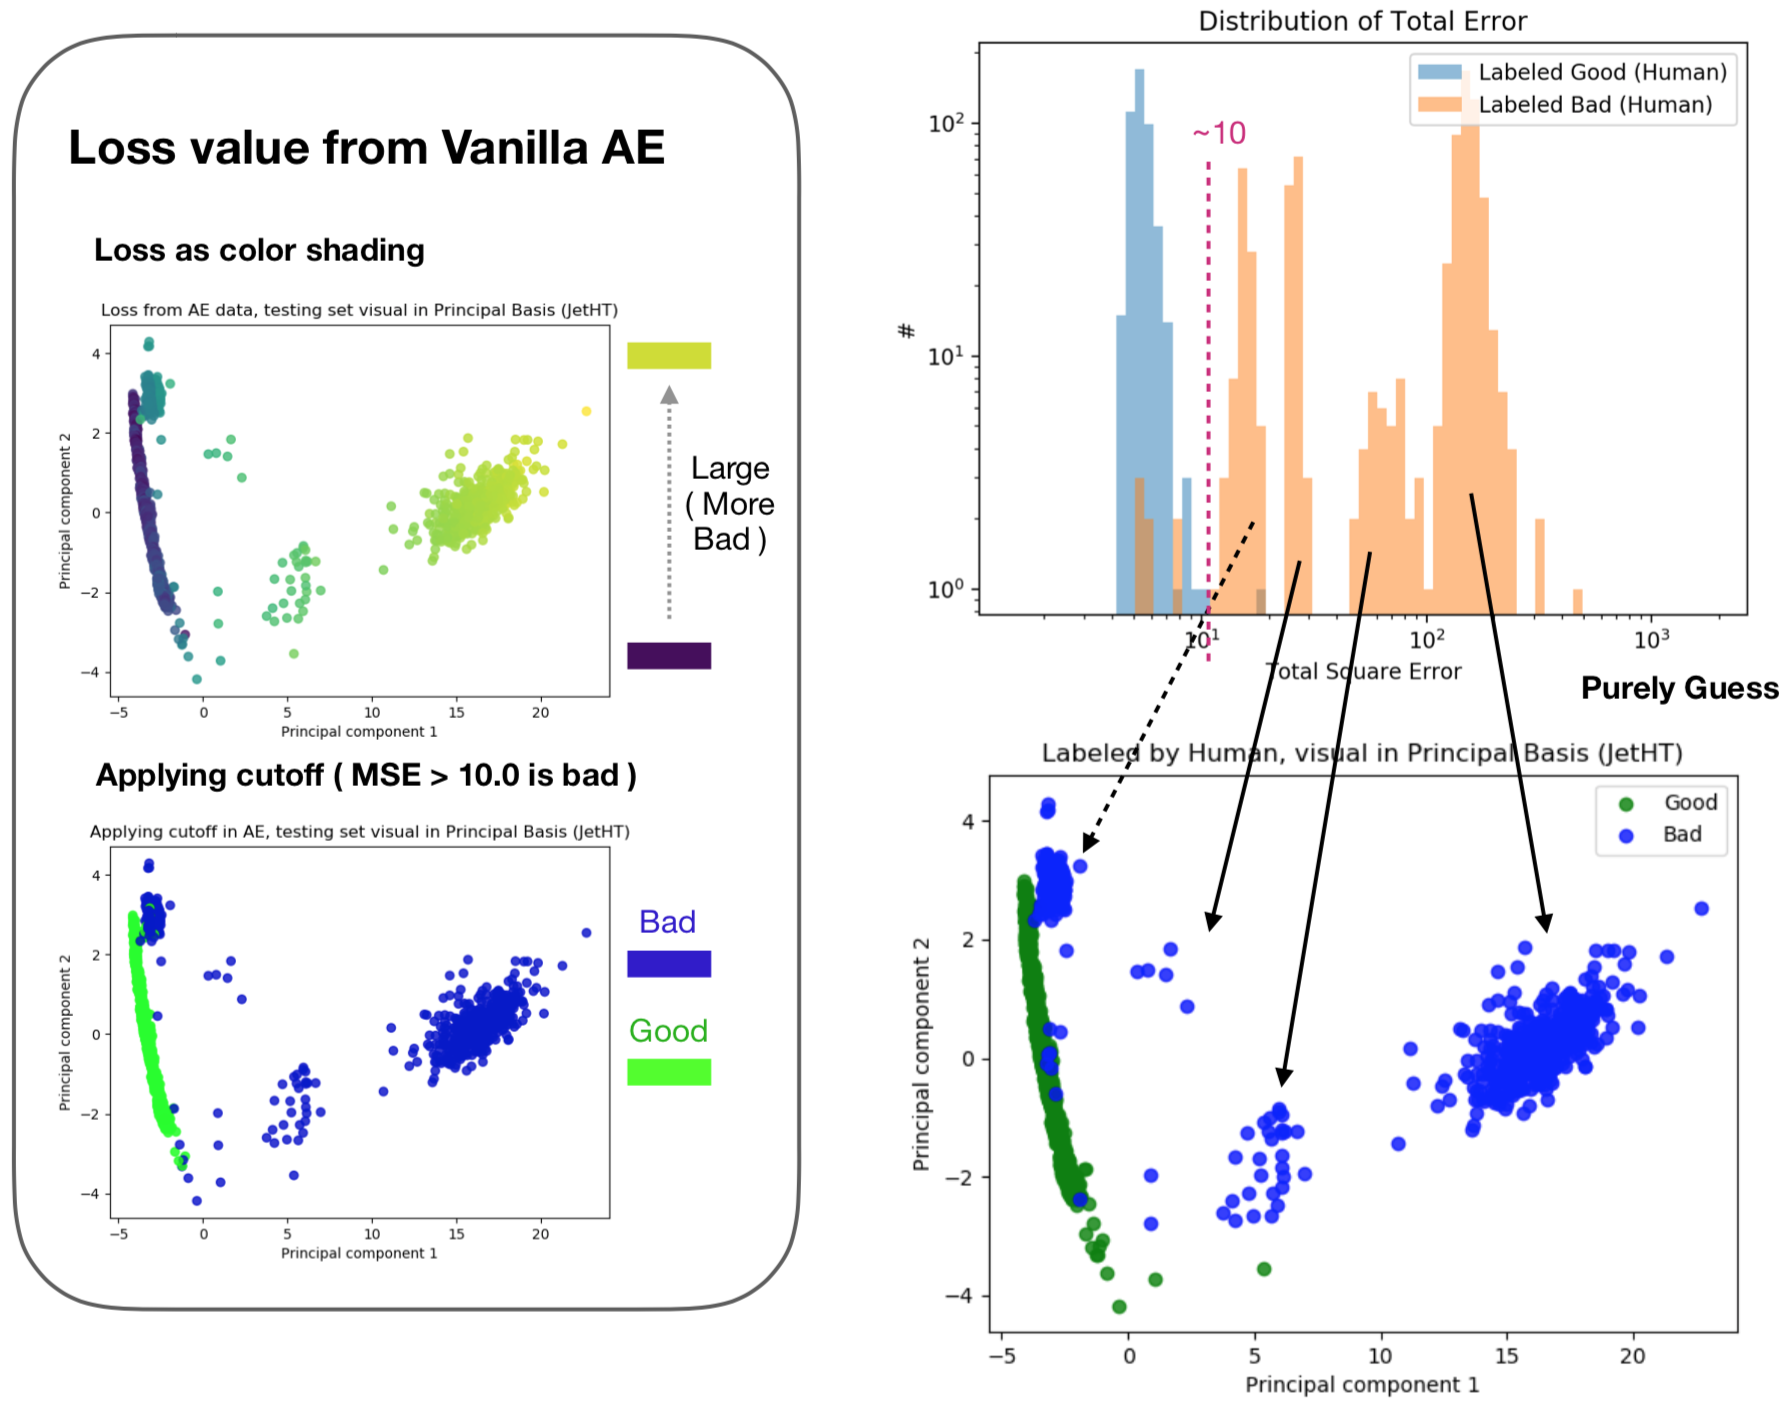
\includegraphics[width=\textwidth]{images/reco/2016/guess_visual.png}
    \caption{Colorize reconstruction error from Vanilla AE}
    \label{fig:2016_guess_visual}
\end{figure}


%%%%%%%%%%%%%%%%%
%     2018
%%%%%%%%%%%%%%%%%

\section{2018 Datasets}

\subsection{Primary Analysis}
For 2018 data, we dig a bit more to understand which cause the badness of bad LS by taking sub-system label into account from RR's API. There are a plenty of sub-system in CMS detector. In order to roughly understand the malfunction of sub-system, we decided to pull label only for HCAL, ECAL, TRACKER and MUON detector which are the main part of the detector.

\begin{figure}[h!]
\centering
    \begin{subfigure}[b]{0.49\linewidth}
        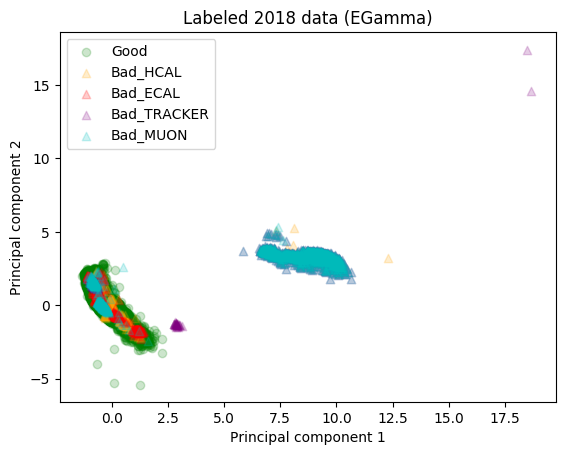
\includegraphics[width=\linewidth]{images/reco/2018/EGamma_subsystem_label.png}
        \caption{Full range}
    \end{subfigure}
    \begin{subfigure}[b]{0.49\linewidth}
        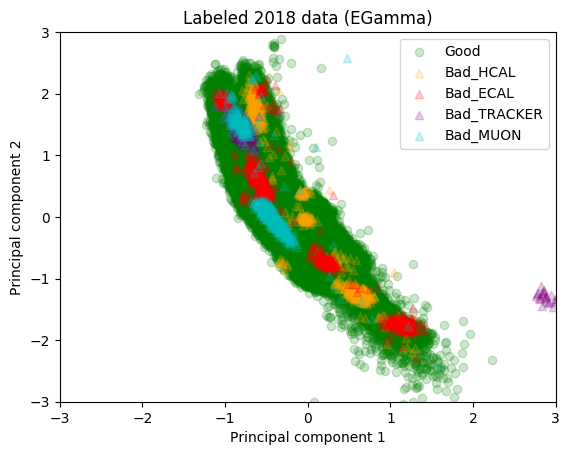
\includegraphics[width=\linewidth]{images/reco/2018/EGamma_subsystem_label_short_range.png}
        \caption{Zoom in}
    \end{subfigure}
\caption{Two principal component of EGamma}
\label{fig:2018_EGamma_subsystem_label}
\end{figure}

\begin{figure}[h!]
\centering
    \begin{subfigure}[b]{0.49\linewidth}
        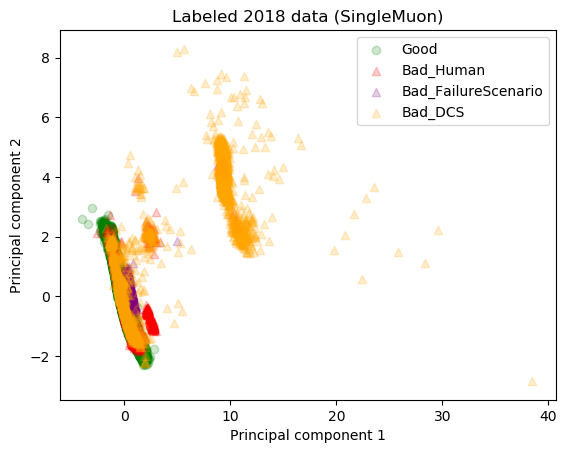
\includegraphics[width=\linewidth]{images/reco/2018/SingleMuon_label_separate.png}
        \caption{Full range}
    \end{subfigure}
    \begin{subfigure}[b]{0.49\linewidth}
        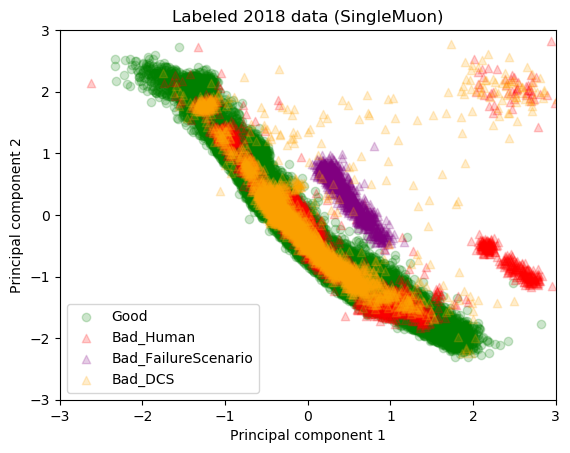
\includegraphics[width=\linewidth]{images/reco/2018/SingleMuon_label_separate_short_range.png}
        \caption{Zoom in}
    \end{subfigure}
    \begin{subfigure}[b]{0.49\linewidth}
        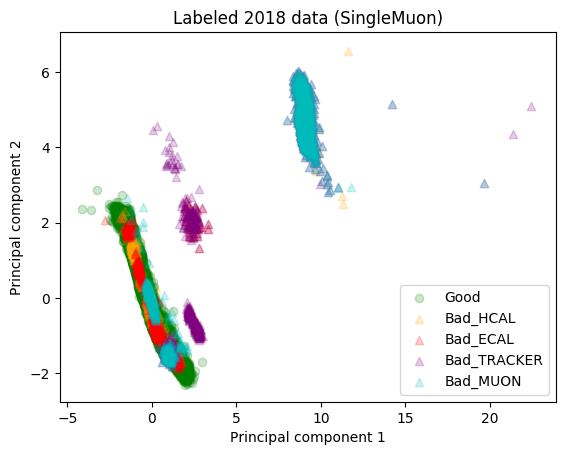
\includegraphics[width=\linewidth]{images/reco/2018/SingleMuon_subsystem_label.png}
        \caption{Full range}
    \end{subfigure}
    \begin{subfigure}[b]{0.49\linewidth}
        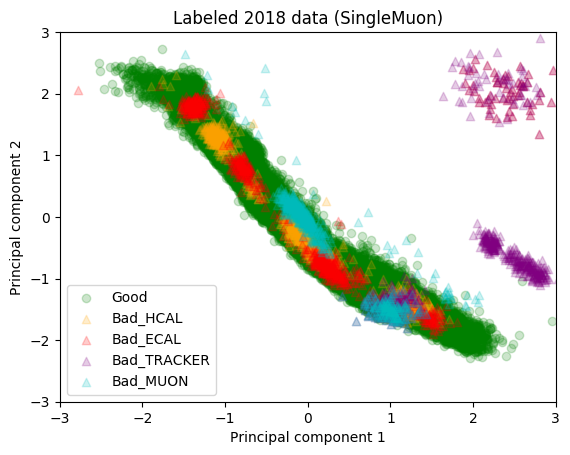
\includegraphics[width=\linewidth]{images/reco/2018/SingleMuon_subsystem_label_short_range.png}
        \caption{Zoom in}
    \end{subfigure}
    \caption{Two principal component of Single Muon}
\label{fig:2018_SingleMuon_subsystem_label}
\end{figure}


\begin{figure}[h!]
\centering
    \begin{subfigure}[b]{0.49\linewidth}
        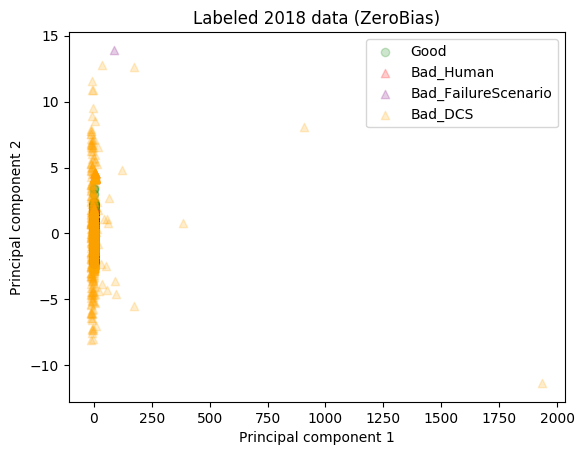
\includegraphics[width=\linewidth]{images/reco/2018/ZeroBias_label_separate.png}
        \caption{Full range}
    \end{subfigure}
    \begin{subfigure}[b]{0.49\linewidth}
        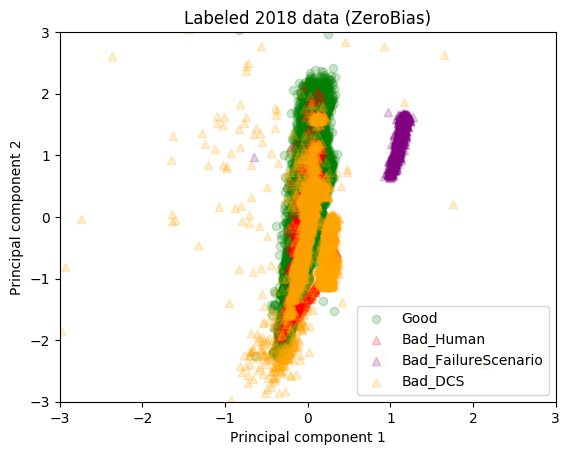
\includegraphics[width=\linewidth]{images/reco/2018/ZeroBias_label_separate_short_range.png}
        \caption{Zoom in}
    \end{subfigure}
    \begin{subfigure}[b]{0.49\linewidth}
        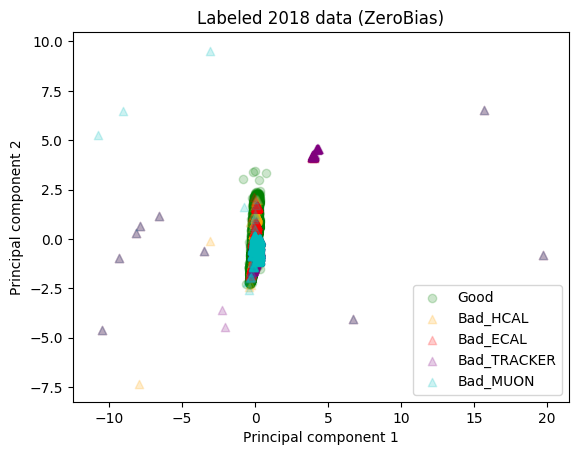
\includegraphics[width=\linewidth]{images/reco/2018/ZeroBias_subsystem_label.png}
        \caption{Full range}
    \end{subfigure}
    \begin{subfigure}[b]{0.49\linewidth}
        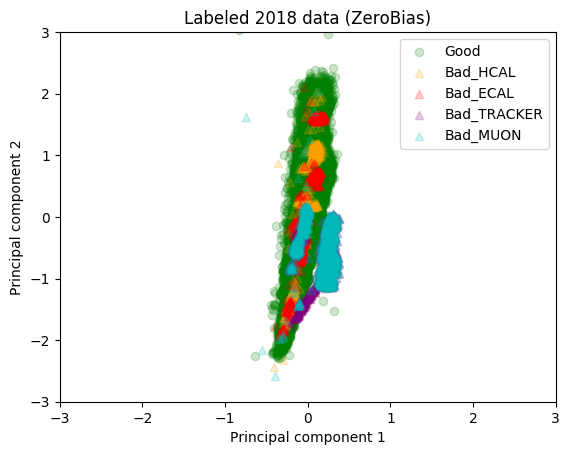
\includegraphics[width=\linewidth]{images/reco/2018/ZeroBias_subsystem_label_short_range.png}
        \caption{Zoom in}
    \end{subfigure}
    \caption{Two principal component of ZeroBias}
\label{fig:2018_ZeroBias_subsystem_label}
\end{figure}

\begin{figure}[h!]
\centering
    \begin{subfigure}[b]{0.49\linewidth}
        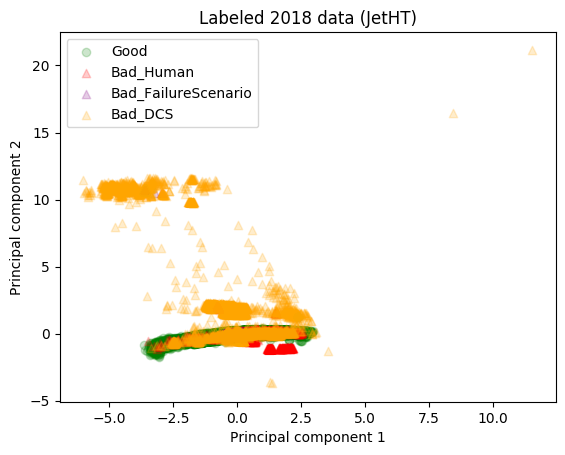
\includegraphics[width=\linewidth]{images/reco/2018/JetHT_label_separate.png}
        \caption{Full range}
    \end{subfigure}
    \begin{subfigure}[b]{0.49\linewidth}
        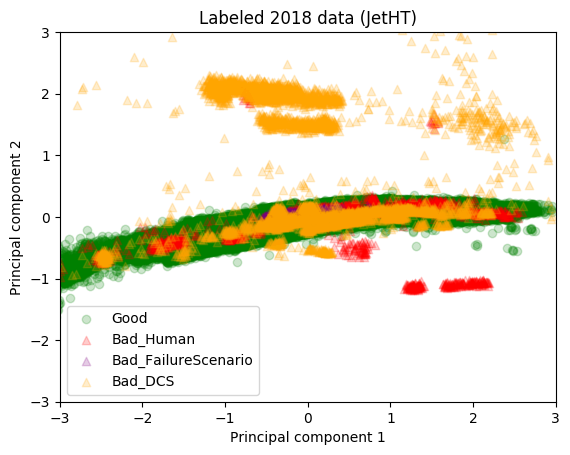
\includegraphics[width=\linewidth]{images/reco/2018/JetHT_label_separate_short_range.png}
        \caption{Zoom in}
    \end{subfigure}
    \begin{subfigure}[b]{0.49\linewidth}
        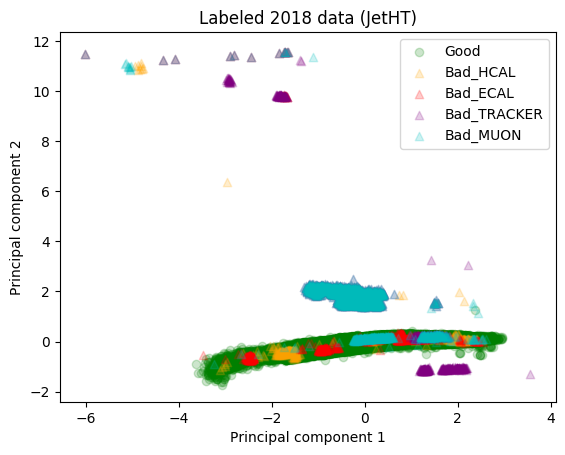
\includegraphics[width=\linewidth]{images/reco/2018/JetHT_subsystem_label.png}
        \caption{Full range}
    \end{subfigure}
    \begin{subfigure}[b]{0.49\linewidth}
        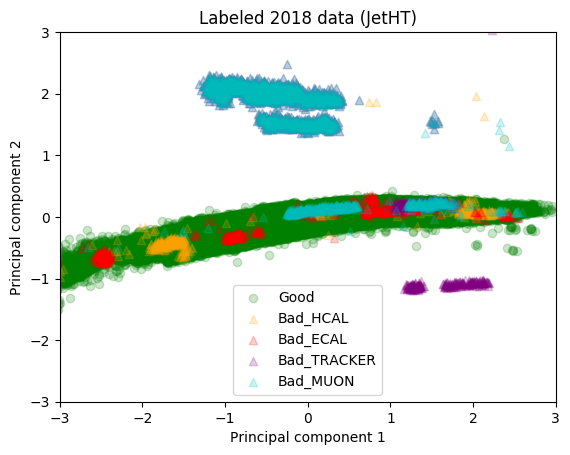
\includegraphics[width=\linewidth]{images/reco/2018/JetHT_subsystem_label_short_range.png}
        \caption{Zoom in}
    \end{subfigure}
    \caption{Two principal component of JetHT}
\label{fig:2018_JetHT_subsystem_label}
\end{figure}

According to Figure (\ref{fig:2018_EGamma_subsystem_label}, \ref{fig:2018_SingleMuon_subsystem_label}, \ref{fig:2018_ZeroBias_subsystem_label}, \ref{fig:2018_JetHT_subsystem_label}), It's obviously to tell that the cluster of outlier are mainly consists of malfunction from MUON and TRACKER sub-detector. Not only the outlier that has an interesting patterns but clustering in inlier is also remarkably considerable as clustering mainly from malfunction of ECAL and HCAL that located near or inside the green band.

Please note that calculation of the matrix transform exclude failure scenario since it's a fake data and it might leading to a weird correlation in covariance matrix.

\subsection{Performance}
\subsubsection{1) Include low statistics (Fill null with zero) and testing with only bad LS form human}
Train with feature set 1 and the result has shown in Figure \ref{fig:2018_f1_ae_performance}.

The performance of AE for EGamma primary dataset is totally inefficient and even worse than randomly picking up which means that model even saw most of bad LS even looks better than many of good LS in the testing datasets. The rest of them is fairly acceptable but still not eought to exploit in the real system. Another interesting spot is the performance between couple of AE in SingleMuon PD. 

\begin{figure}[h!]
\centering
    \begin{subfigure}[b]{0.49\linewidth}
        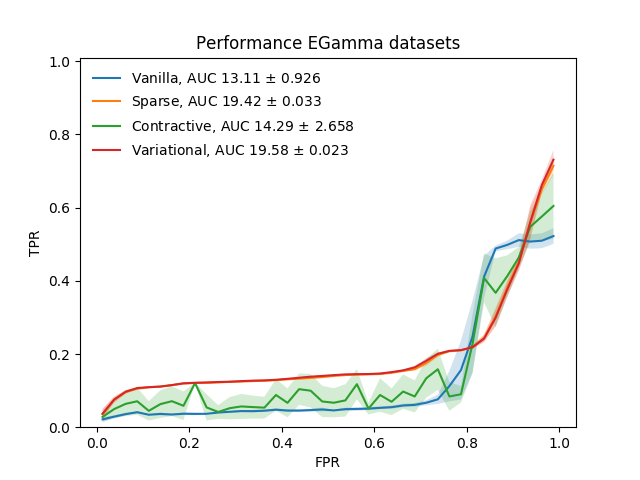
\includegraphics[width=\linewidth]{images/reco/2018/feature_1/performance_EGamma_VanillaSparseContractiveVariational.png}
        \caption{EGamma}
    \end{subfigure}
    \begin{subfigure}[b]{0.49\linewidth}
        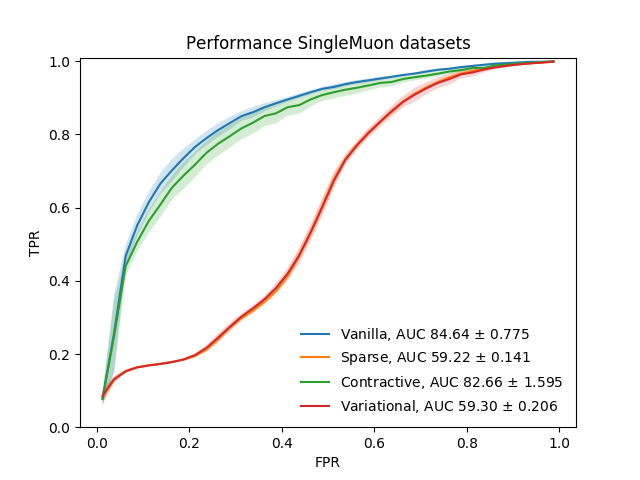
\includegraphics[width=\linewidth]{images/reco/2018/feature_1/performance_SingleMuon_VanillaSparseContractiveVariational.png}
        \caption{SingleMuon}
    \end{subfigure}
    \begin{subfigure}[b]{0.49\linewidth}
        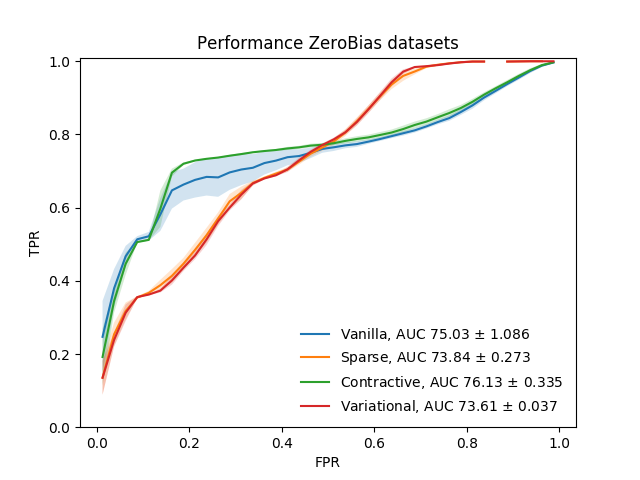
\includegraphics[width=\linewidth]{images/reco/2018/feature_1/performance_ZeroBias_VanillaSparseContractiveVariational.png}
        \caption{ZeroBias}
    \end{subfigure}
    \begin{subfigure}[b]{0.49\linewidth}
        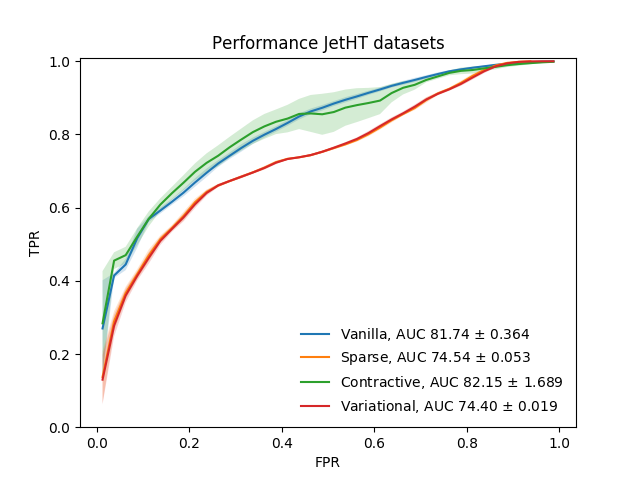
\includegraphics[width=\linewidth]{images/reco/2018/feature_1/performance_JetHT_VanillaSparseContractiveVariational.png}
        \caption{JetHT}
    \end{subfigure}
    \caption{Model performance for feature set 1 with 2018 data}
\label{fig:2018_f1_ae_performance}
\end{figure}

Figure \ref{fig:2018_f1_exteded_ae_performance} has demonstrated that even extended model has been combined various constrains that we known but it is still not improve any further in term of performance. Nevertheless, it has a remarkable stability especially for ContractiveVariational AE.

\begin{figure}[h!]
\centering
    \begin{subfigure}[b]{0.49\linewidth}
        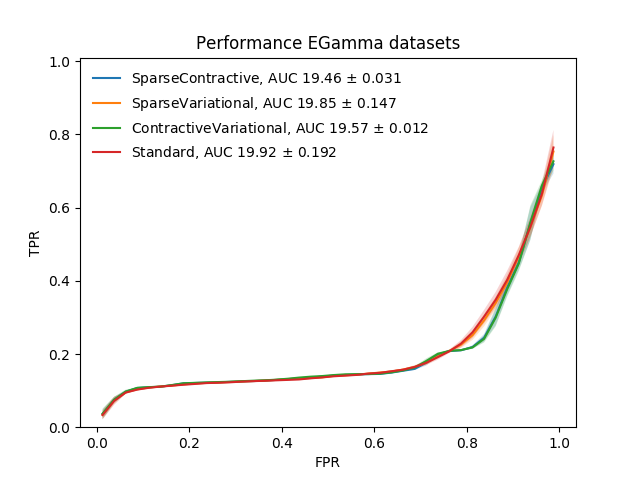
\includegraphics[width=\linewidth]{images/reco/2018/feature_1/performance_EGamma_SparseContractiveSparseVariationalContractiveVariationalStandard.png}
        \caption{EGamma}
    \end{subfigure}
    \begin{subfigure}[b]{0.49\linewidth}
        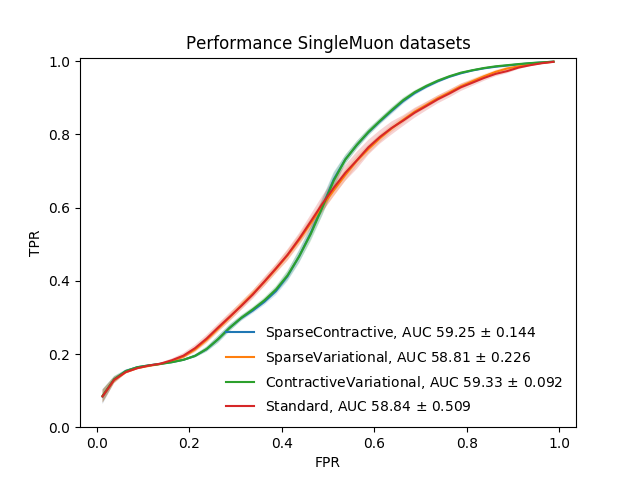
\includegraphics[width=\linewidth]{images/reco/2018/feature_1/performance_SingleMuon_SparseContractiveSparseVariationalContractiveVariationalStandard.png}
        \caption{SingleMuon}
    \end{subfigure}
    \begin{subfigure}[b]{0.49\linewidth}
        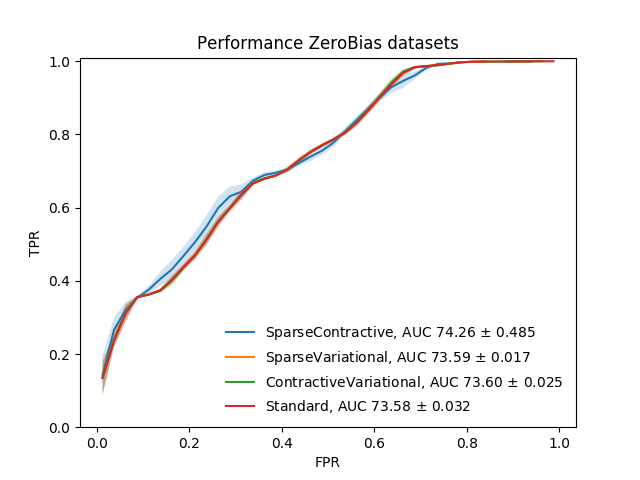
\includegraphics[width=\linewidth]{images/reco/2018/feature_1/performance_ZeroBias_SparseContractiveSparseVariationalContractiveVariationalStandard.png}
        \caption{ZeroBias}
    \end{subfigure}
    \begin{subfigure}[b]{0.49\linewidth}
        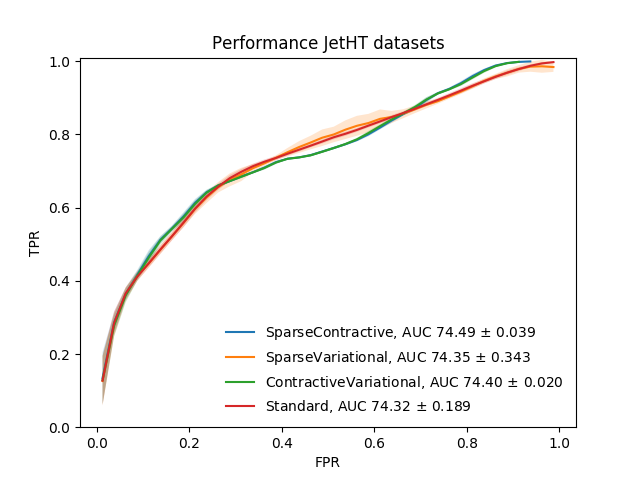
\includegraphics[width=\linewidth]{images/reco/2018/feature_1/performance_JetHT_SparseContractiveSparseVariationalContractiveVariationalStandard.png}
        \caption{JetHT}
    \end{subfigure}
    \caption{Extended model performance for feature set 1 with 2018 data}
\label{fig:2018_f1_exteded_ae_performance}
\end{figure}


\subsubsection{2) Exclude low statistics (Filter LS that has low EventsPerLs with value in the settings)}
Train with feature set 1 and the result has shown in Figure \ref{fig:2018_f2_ae_performance}.


\begin{figure}[h!]
\centering
    \begin{subfigure}[b]{0.49\linewidth}
        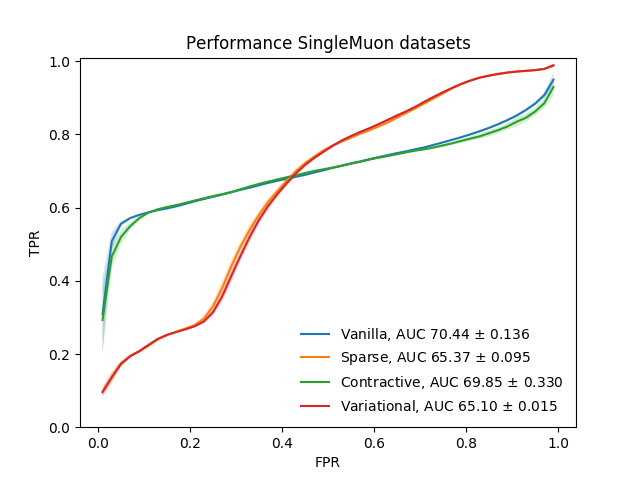
\includegraphics[width=\linewidth]{images/reco/2018/feature_2/performance_SingleMuon_VanillaSparseContractiveVariational.png}
        \caption{Full range}
    \end{subfigure}
    \begin{subfigure}[b]{0.49\linewidth}
        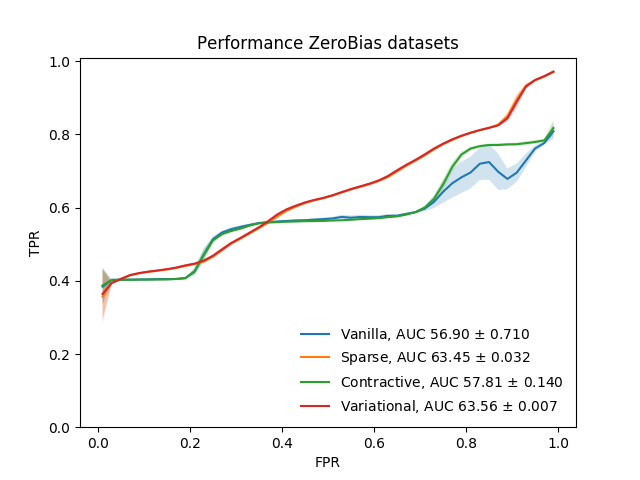
\includegraphics[width=\linewidth]{images/reco/2018/feature_2/performance_ZeroBias_VanillaSparseContractiveVariational.png}
        \caption{Zoom in}
    \end{subfigure}
    \begin{subfigure}[b]{0.49\linewidth}
        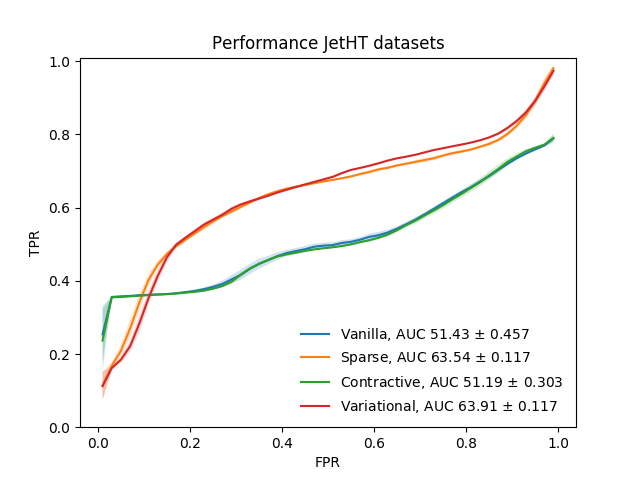
\includegraphics[width=\linewidth]{images/reco/2018/feature_2/performance_JetHT_VanillaSparseContractiveVariational.png}
        \caption{Full range}
    \end{subfigure}
    % \begin{subfigure}[b]{0.49\linewidth}
    %     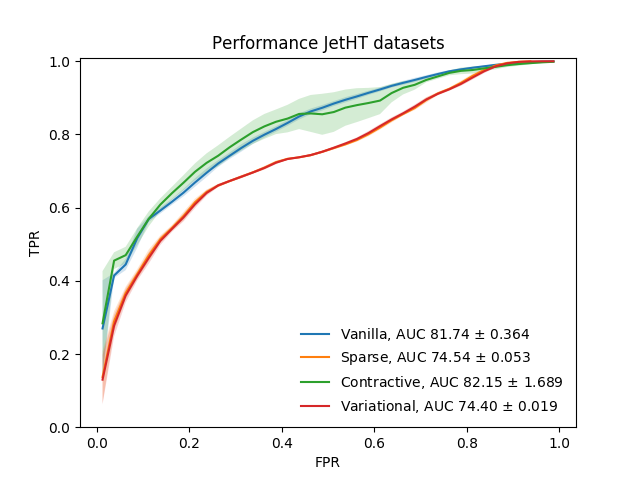
\includegraphics[width=\linewidth]{images/reco/2018/feature_1/performance_JetHT_VanillaSparseContractiveVariational.png}
    %     \caption{Zoom in}
    % \end{subfigure}
    \caption{Model performance for feature set 2 with 2018 data}
\label{fig:2018_f2_ae_performance}
\end{figure}

\subsubsection{Distribution of decision value (to find the threshold)}

\begin{figure}[h!]
\centering
    \begin{subfigure}[b]{0.49\linewidth}
        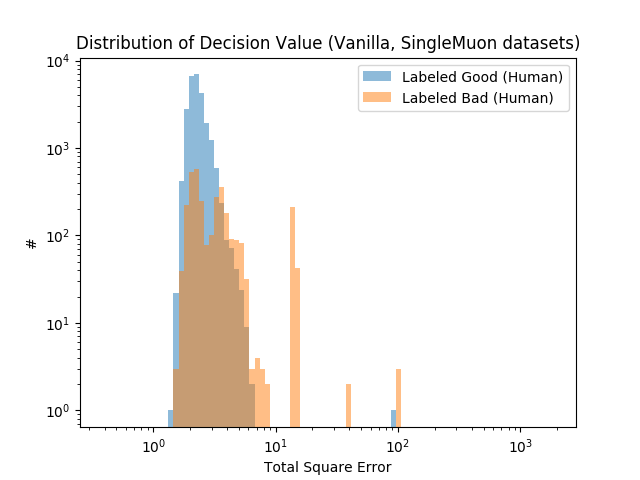
\includegraphics[width=\linewidth]{images/reco/2018/feature_2/se_dist_Vanilla1f2_SingleMuon.png}
        \caption{SingleMuon}
    \end{subfigure}
    \begin{subfigure}[b]{0.49\linewidth}
        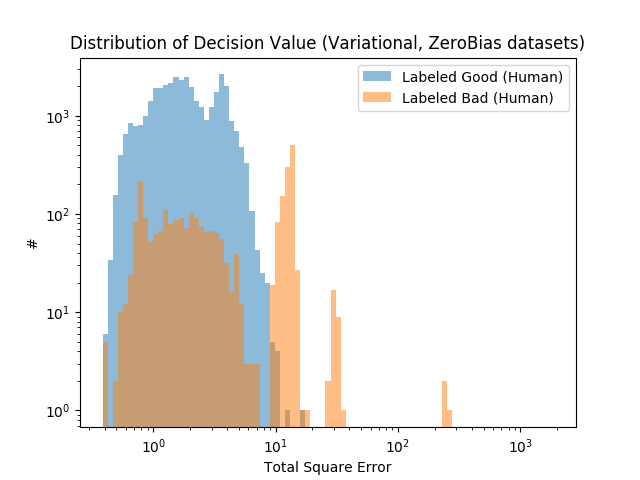
\includegraphics[width=\linewidth]{images/reco/2018/feature_2/se_dist_Variational1f2_ZeroBias.png}
        \caption{ZeroBias}
    \end{subfigure}
    \begin{subfigure}[b]{0.49\linewidth}
        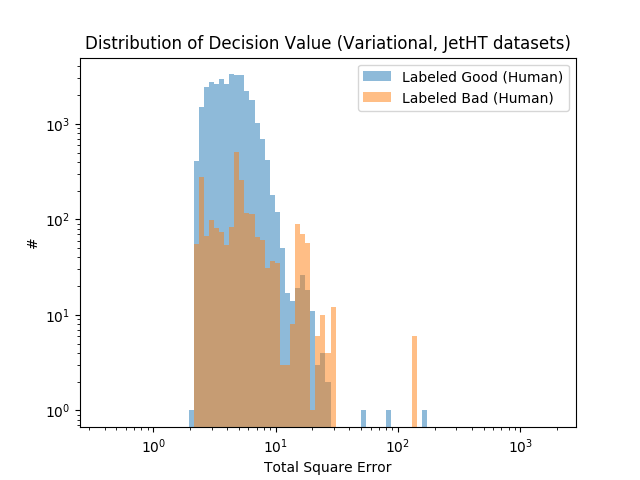
\includegraphics[width=\linewidth]{images/reco/2018/feature_2/se_dist_Variational1f2_JetHT.png}
        \caption{JetHT}
    \end{subfigure}
    \caption{Distribution of decision value}
\label{fig:2018_f2_se_dist}
\end{figure}